\documentclass[sigconf]{acmart}

\usepackage{hyperref}
\usepackage{graphicx}
\graphicspath{ {images/} }
\usepackage{endfloat}
\renewcommand{\efloatseparator}{\mbox{}} % no new page between figures

\usepackage{booktabs} % For formal tables

\settopmatter{printacmref=false} % Removes citation information below abstract
\renewcommand\footnotetextcopyrightpermission[1]{} % removes footnote with conference information in first column
\pagestyle{plain} % removes running headers

\begin{document}
\title{Big Data Analytics for Municipal Waste Management}

\author{Andres Castro Benavides}
\orcid{1234-5678-9012}
\affiliation{%
  \institution{Indiana University}
  \streetaddress{107 S. Indiana Avenue}
  \city{Bloomington} 
  \state{Indiana} 
  \postcode{43017-6221}
}
\email{acastrob@iu.edu}

\author{Mani Kumar Kagita}
\affiliation{%
  \institution{Indiana University}
  \streetaddress{107 S. Indiana Avenue}
  \city{Bloomington} 
  \state{Indiana} 
  \postcode{43017-6221}
}
\email{mkagita@iu.edu}
% The default list of authors is too long for headers}
\renewcommand{\shortauthors}{B. Trovato et al.}


\begin{abstract}
As waste management becomes a greater concern for cities and municipalities around the world with increase in population and the waste, big data analysis has the potential to not only help assess the current waste management strategies but also provide information that can be used to optimize the systems used in various institutions, local government, companies, etc.

\end{abstract}

\keywords{Waste Management, Big Data, Local Government}


\maketitle

\section{Introduction}


In the current fast paced society, as production of goods increases and new distribution chains constantly change, the production of disposed materials and goods, from now on called solid waste, has increased over the past ten years, going from around 0.64 kg per person per day of solid waste to approximately 1.2 kg per person per day,  and it is expected to increase to about 1.42 kg by 2025.
~\cite{hoornweg2012} This causes the problem of waste management to increase in complexity and magnitude.

Because of this, different local governments and organizations have seen the need to develop regulations to control the different features, segments, processes of the action of disposal from the moment the material is discarded until the moment the material reaches it's ultimate destination like recycling plant or landfill. This set of systematic regulations is called solid waste management. Simple techniques are used in earlier days to make decisions for waste management which is to choose an option from multiple available options  ~\cite{akbarpour2016}. Decision-making became much more complex when multiple parameters adds up to the system.

Classifications of solid waste is determined by its sources, various types of wastes accumulated and the rate of disposal are to be constantly monitored and controlled in parallel along with improving current systems ~\cite{chandrappa2012}. Large volumes of data will be collected on daily basis from each classification of solid waste which includes multiple parameters. Multivariate data analysis methods ~\cite{bohm2013} provides an exploratory data analysis, classification and parameter prediction using this data.


\section{ Municipal Solid Waste Management}
%a) what is the problem

Municipal Solid Waste (MSW) commonly termed as the garbage or trash consists of items we use in everyday life like food leftovers, plastic bottles, wooden furniture, electrical and electronic appliances, glass, medical waste, cardboards, waste tires, office wastes, consumer goods etc which comes from residential, commercial, institutional and industrial sites. 

The amounts of disposed material and it's composition vary depending on the country, place and activity that is performed at the site where the waste is generated ~\cite{chandrappa2012}. According to EPA statistics 2014, Americans have generated about 258 million tons of MSW in which more than 89 million tons is recycled and composted. This is equivalent to 34.6\% recycling rate compared to 6.4\% in 1960. In addition, 33 million tons of trash is combusted for energy and 136 million tons were landfilled. Figures below represents MSW generation rates, recycling, composition rates and Total MSW generation between 1960 and 2014 ~\cite{EPA2014}.

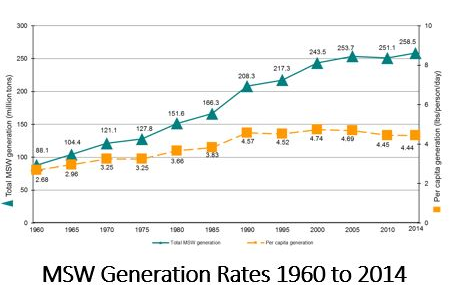
\includegraphics[width=8cm, height=7cm]{fig1.png}


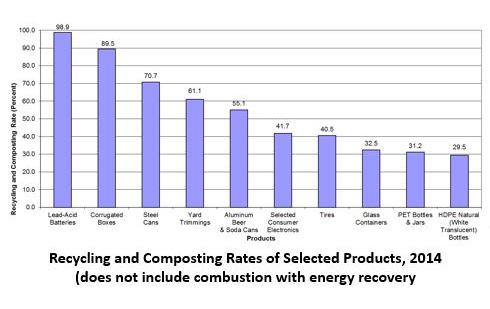
\includegraphics[width=8cm, height=7cm]{fig2.png}


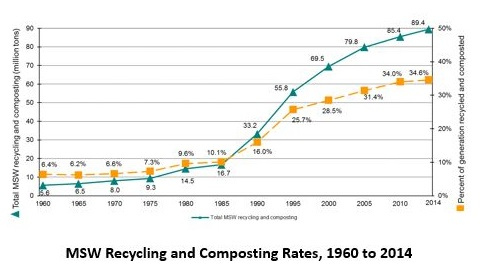
\includegraphics[width=8cm, height=7cm]{fig3.jpg}


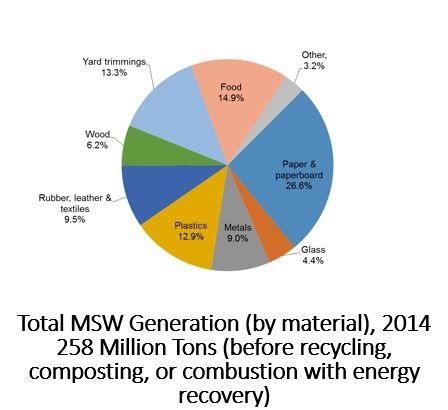
\includegraphics[width=8cm, height=7cm]{fig4.jpg}


There are also important differences between the general composition of the waste generated in rural area and what is produced in urban area, the waste produced in the later is highly influenced by the culture and the practices of our modern society.~\cite{chandrappa2012}


For this reason, every process related to waste management-transportation, storing and final disposition, among others- must be engineered and tailored to fit the specific needs of each case.



In general, decisions can be classified as optimal, good, or fortuitous. ~\cite{akbarpour2016} and this can be applied to Waste Management.

Having that Good decision-making is mostly based on experience, comparison of elements and trial and error, and that fortuitous decision-making have no scientific base; one must always try to solve the problem -in this case waste management related- with Optimal Decision making, that requires techniques and technologies provided by other fields. 
 ~\cite{akbarpour2016}


\section{ Big data and waste management}
%b) why is big data involved
By collecting and storing large volumes of  data related to types of waste, quantities, periodicity, and composition; usually from independent sources. Big data can be interpreted in a way that allows the different actors that intervene in Waste Management to make Optimal Decisions.~\cite{yenkar2014review} Big Data refers to taking very large amount of data sets and applying technologies to analyze these data sets. As stated in ''Fourth Paradigm'' ~\cite{hey2009fourth}, big data exploration is about finding patterns in data, analyzing the trends and causalities.

Big Data can be used for strategic policy making in almost any field and the Greater Manchester Waste Disposal Authority (GMWDA), England's largest Waste Disposal Authority, has turned Big Data to better plan their services. In order to achieve that, they are collaborating with the University of Manchester who uses the data generated by the GMWDA. Together they help create environmentally sustainable solutions for Manchester and the 1.1 million tonnes of waste that is produced each year ~\cite{markvan2016}. 

Big data will help governments to track the amount of disposals at different locations and their quantity in-order to generate heat maps of locations with largest waste collected and will help to improve necessary solutions for better environments~\cite{markvan2016}. Waste Management is not only government issue. Citizens should take initiative and educate others on how to recycle waste for their better living. With the help of collected data, governments will notify citizens about the importance of waste management through mobile phones as its considered the cheapest means of communication in modern world.

%we can add info about how it is collected and stored? Sources and uses? Integrated Waste management plans ordered by law in many countries?

\subsection{Solutions for effective Waste Management}
%how can big data or analytics of big data help


Purpose of Big data in waste management is to facilitate municipal government bodies on how much waste is disposed, environmental pollution, rate at which waste is recycled, optimizing routes to reduce the time and money.

One such solution is being implemented in an upcoming smart city of Songdo, a chip card is made mandatory for every citizen to use while disposing their garbage. Data collected from these chip cards will be used for analyzing on the quantity of waste disposed, and their locations. Each trash bin is incorporated with sensors to provide height of the garbage accumulated, temperature and air pollution levels. These multiple parameters help municipal authorities to forecast perfect timings to collect the trash and optimize the routes to save time and their cost ~\cite{markvan2016}.

Researchers in Ethiopia are combining socioeconomic data along with geographic data to get a clear understanding on the patterns of how household waste is being properly distributed and collected. This study helped local authorities to better manage waste practices in urban areas~\cite{markvan2016}. 

A group of researcher from University of Stockholm are using Big Data to identify on how the transportation of waste and the garbage collection routes can be optimized in the city. Using wide variety of data sets collected from various sources, roughly around half a million entries of waste fractions(as showin in fig below), trash bin locations, weights, truck routes researchers have develop waste generation maps of Stockholm. This research help to reveal quite a few inefficiencies the local government is facing and help to improve the waste management ~\cite{markvan2016}.

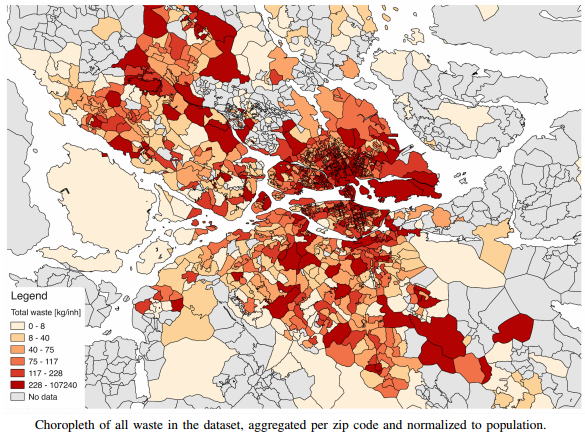
\includegraphics[width=8cm, height=6cm]{stockholm.png}


\subsubsection{Vehicle Routing Problem}
Vehicle route optimization is one of the main concern in waste management. It is generally termed as Vehicle Routing Problem(VRP) ~\cite{Dantzig1959}. Given a common problem to a general heuristic a strong solutions can be modeled manually to solve it. But in a real-world multiple factors will be influenced either directly or indirectly to that problem. Common known factors that shows influence on vehicle routing problems are number of vehicles, garbage collection stops and the route length. Depending on the complexity of problem, few more factors can be included like vehicle types and disposal facilities. 

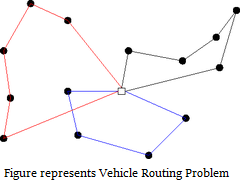
\includegraphics[width=8cm, height=6cm]{vrp}


Two of the most basic VRPs are the Travelling Salesman Problem (TSP) and the Chinese Postman Problem (CPP) according to Joroen, Liesje and Jonas ~\cite{Beliën2012}. But when too many constraints and attributes are considered, both of the TSP and CPP tends to get harder to solve problems. Many researchers had made various publications since 1995 on waste management vehicle routing problems as shown in Figure 1 and yet the problem still persists. Mathematical models need to be developed to provide city administrators with a tool to make effective long-and short-term decisions relating to their municipal disposal system ~\cite{Bhat1996}. 

In modern world, not only direct impacted attributes causing VRP problems. But indirect attributes like daily traffic, weather conditions, energy prices, demand fluctuations, vehicle health, dump site inventory also affecting to strengthen the worst. Research team at OSI came up with a better solution for solving VRP problems using Big Data technologies. Mixed Integer Programming (MIP) formulation interacts with millions of attributes in a live environments providing real-time decisions to optimize the VRP. Big Data technologies are used to enable prediction of travel times, address demand forecasting on a tactical time horizon. This approach showed a tremendous improvement in forecasting part of the VRP problem at a range of 5\% to 10\% ~\cite{vijay2013}. Any improvement, even less than 5\% created on VRP is a significant improvement ~\cite{Hasle2007}.

In 2011, Faccio, Persona and Zanin ~\cite{faccio2011} investigated the feasibility of communication between bins, collection vehicles and a central operator. The waste bins can be fitted with a volumetric sensor, RFID and GPRS communication and can send information about their status. Using this real-time data, routes can be optimized in order to make optimal use of the vehicle's cargo space. Waste containers that still have not reached a certain threshold to be emptied are skipped by, saving valuable travel time and distance. Also of importance, fewer waste collection vehicles were needed. A key finding was that the economic feasibility of providing a sensor network to support waste management in this case, was estimated to a payback period of roughly three years ~\cite{shahrokni2014big}.

Real-time, on-demand routing is helping now to address operating costs and service improvements. Trash collection vehicles are closely monitored with a remote self-diagnostics to identify vehicle health, required repairs and pre-ordering of replacement parts. This will help to prevent downtime of garbage collection trucks from being getting repairs. Hand-held applications and tools for autonomous service verification are being used in measuring program success and to outreach programs ~\cite{Megan2017}.


\subsubsection{Disposal of Landfills Problem}

The process of solving a math program requires a large number of calculations and is, therefore, best performed by a computer program. ~\cite{akbarpour2016}

\section{Opportunities for Waste Management Optimization}

%what infrastructure/programs/systems exist for this

\subsection{Statistics and Waste Management}

There are many data analysis methods that are used when studying waste management, but the two most popular are PCA and PLS1. 
~\cite{bohm2013}

Lingo is a mathematical modeling language designed particularly for formulating and solving a wide variety of optimization problems including linear programing. Lingo optimization software uses branch and bound methods to solve problems of this type. ~\cite{akbarpour2016}

\subsection{GIS Analytics}

When it comes to Geographical Information Systems (From now on GIS) there are multiple software and hardware options in the market. From paid software like ArcGIS to Open and free software like GVSIG, there are solutions that can help interpret large data sets, apply statistics and algorithms of different kinds and display them in a way that make reference to a geographical space. %general knowledge? Should we get a citation for this?

The second category of studies focuses on minimizing transportation of waste collection through optimal routing algorithms. For example Kim et al [18] use two methods to calculate an optimal set of routes, the first being Solomon's insertion algorithm, the second being a clustering algorithm. Their aim was to minimize the driven distance, as well as to balance the workload. At the same time, the constraint of legally prescribed lunch breaks (so called time-window problem) had to be satisfied. McLeod and Cherrett [19] suggested a route optimization for three areas and connected waste companies in North Hampshire (UK). By applying simple rerouting, sharing of routes between the 3 areas and adding vehicle depots at the waste disposal sites, they estimated annual savings as large as 10,000 km for the studied routes (this covers one fifth of all routes in North Hampshire). 

Another study performed by Wy, Kim and Kim [20] studied a routing algorithm for waste collection using roll-on/roll-off containers, again while factoring in the time windows. Buhrkal, Larsen and Ropke [21] were one of the first to suggest the environmental importance of optimizing waste collection itineraries. They utilized an adaptive large neighborhood search algorithm, and a clustering method and their scope was residential waste collection. Depending on the computation time, using the actual collection points and lunch time windows, the savings amounted to 13 percent average. With larger time windows and better starting conditions, heuristics with a distance reduction of up to 45\% could be achieved ~\cite{shahrokni2014big}.


Many data analysis methods are used when studying waste management, but the two most popular are PCA and PLS1. 
~\cite{bohm2013}




\section{Conclusions}

There are different tools to optimize the different waste management practices  and to improve the information available for decision makers.
Local governments had just started to adopt Big Data technologies for solving problems involved in MSW. In future using Big data Analytics, large amounts of data sets will be used to identify trends and patterns that could highlight improvement opportunities. Big Data will play a major lead role in managing better smart cities and government authorities will be benefited with tremendous improvements in waste management. Thanks to Big Data Analytics for making smart cities much more effective and efficient.


\appendix


% This next section command marks the start of
% Appendix B, and does not continue the present hierarchy

% \section{More Help for the Hardy}
\appendix



% This next section command marks the start of
% Appendix B, and does not continue the present hierarchy


%\begin{acks}


%\end{acks}

\bibliographystyle{ACM-Reference-Format}
\bibliography{report} 

\end{document}
